\documentclass[xcolor=svgnames, usepdftitle=false, aspectratio=169]{beamer}
\usepackage{pgfpages}
\setbeameroption{hide notes}

\frenchspacing

% --- THEME ---
\usetheme[progressbar=frametitle]{metropolis}

\useoutertheme{metropolis}
\useinnertheme{metropolis}
\usefonttheme{metropolis}
\usecolortheme{dove}  % spruce, metropolis, dove, crane, beaver, seagull
\setbeamercolor{background canvas}{bg=transparent}
\usecolortheme[named=DarkOrange]{structure}
\usefonttheme[onlymath]{serif}

% \setbeamersize{text margin left=5.03cm}
\setbeamercolor{title separator}{fg=DarkOrange}

% --- HACKS ---
% Hide numbers on standout slides.
\setbeamertemplate{frame numbering}{
    \ifbool{metropolis@standout}{}{
        \insertframenumber
    }
}
\setbeamertemplate{frame numbering}[counter]  % none, counter, fraction

% Avoid font-warning with itemize bullets.
\renewcommand\textbullet{\ensuremath{\bullet}}

% --- PACKAGES ---
\usepackage[UKenglish]{babel}
\usepackage[utf8]{inputenc}
\usepackage{lmodern}
\usepackage[T1]{fontenc}

% \usepackage{appendixnumberbeamer}
\usepackage{upquote}
\usepackage[straightquotes]{newtxtt}
\usetikzlibrary{positioning}
% \usepackage{minted}
\usepackage{multicol}
\usepackage{xspace}
\usepackage{booktabs}
\usepackage{siunitx}

% --- SETTINGS ---
\graphicspath{{../figures/}}
\setlength{\fboxsep}{0pt}

% --- OWN COMMANDS ---
\newcommand{\bdra}{\ensuremath{\boldsymbol \Rightarrow }~}
\newcommand{\bdla}{\ensuremath{\boldsymbol \Leftarrow }~}
\newcommand{\dra}{\ensuremath{\Rightarrow }~}
\newcommand{\dla}{\ensuremath{\Leftarrow }~}
\newcommand{\mr}[1]{\mathrm{#1}}
\newcommand{\emg}[2]{\texttt{emg#1#2}\xspace}
\newcommand{\empymod}{\texttt{empymod}\xspace}
\newcommand{\ohmm}{\ensuremath{\Omega\,}\text{m}\xspace}
\newcommand{\rmk}[1]{{\color{red}\bfseries #1}}
\newcommand{\maybe}[1]{{\color{gray} #1}}
\newcommand{\todo}{{\color{red}\texttt{TODO:}}\xspace}
\newcommand{\bm}[1]{{\mathbf{#1}}}

% --- TITLE-STUFF ---

\newcommand{\ttitle}{Time-domain CSEM modelling}
\title{\vspace{2.5cm}\color{white}{\ttitle}}
\subtitle{\color{white}{using frequency- and Laplace-domain computations}}
\date{\color{white}{20 October 2021}}
\author{\vspace{-.3cm}\color{white}{Dieter Werthmüller and Evert Slob, TU Delft}}
\institute{}

\hypersetup{pdftitle={\ttitle}, allcolors=NavyBlue, colorlinks=true}

% --- SLIDES ---
\begin{document}
\metroset{block=fill}  % Fills the block-environment
\usebackgroundtemplate{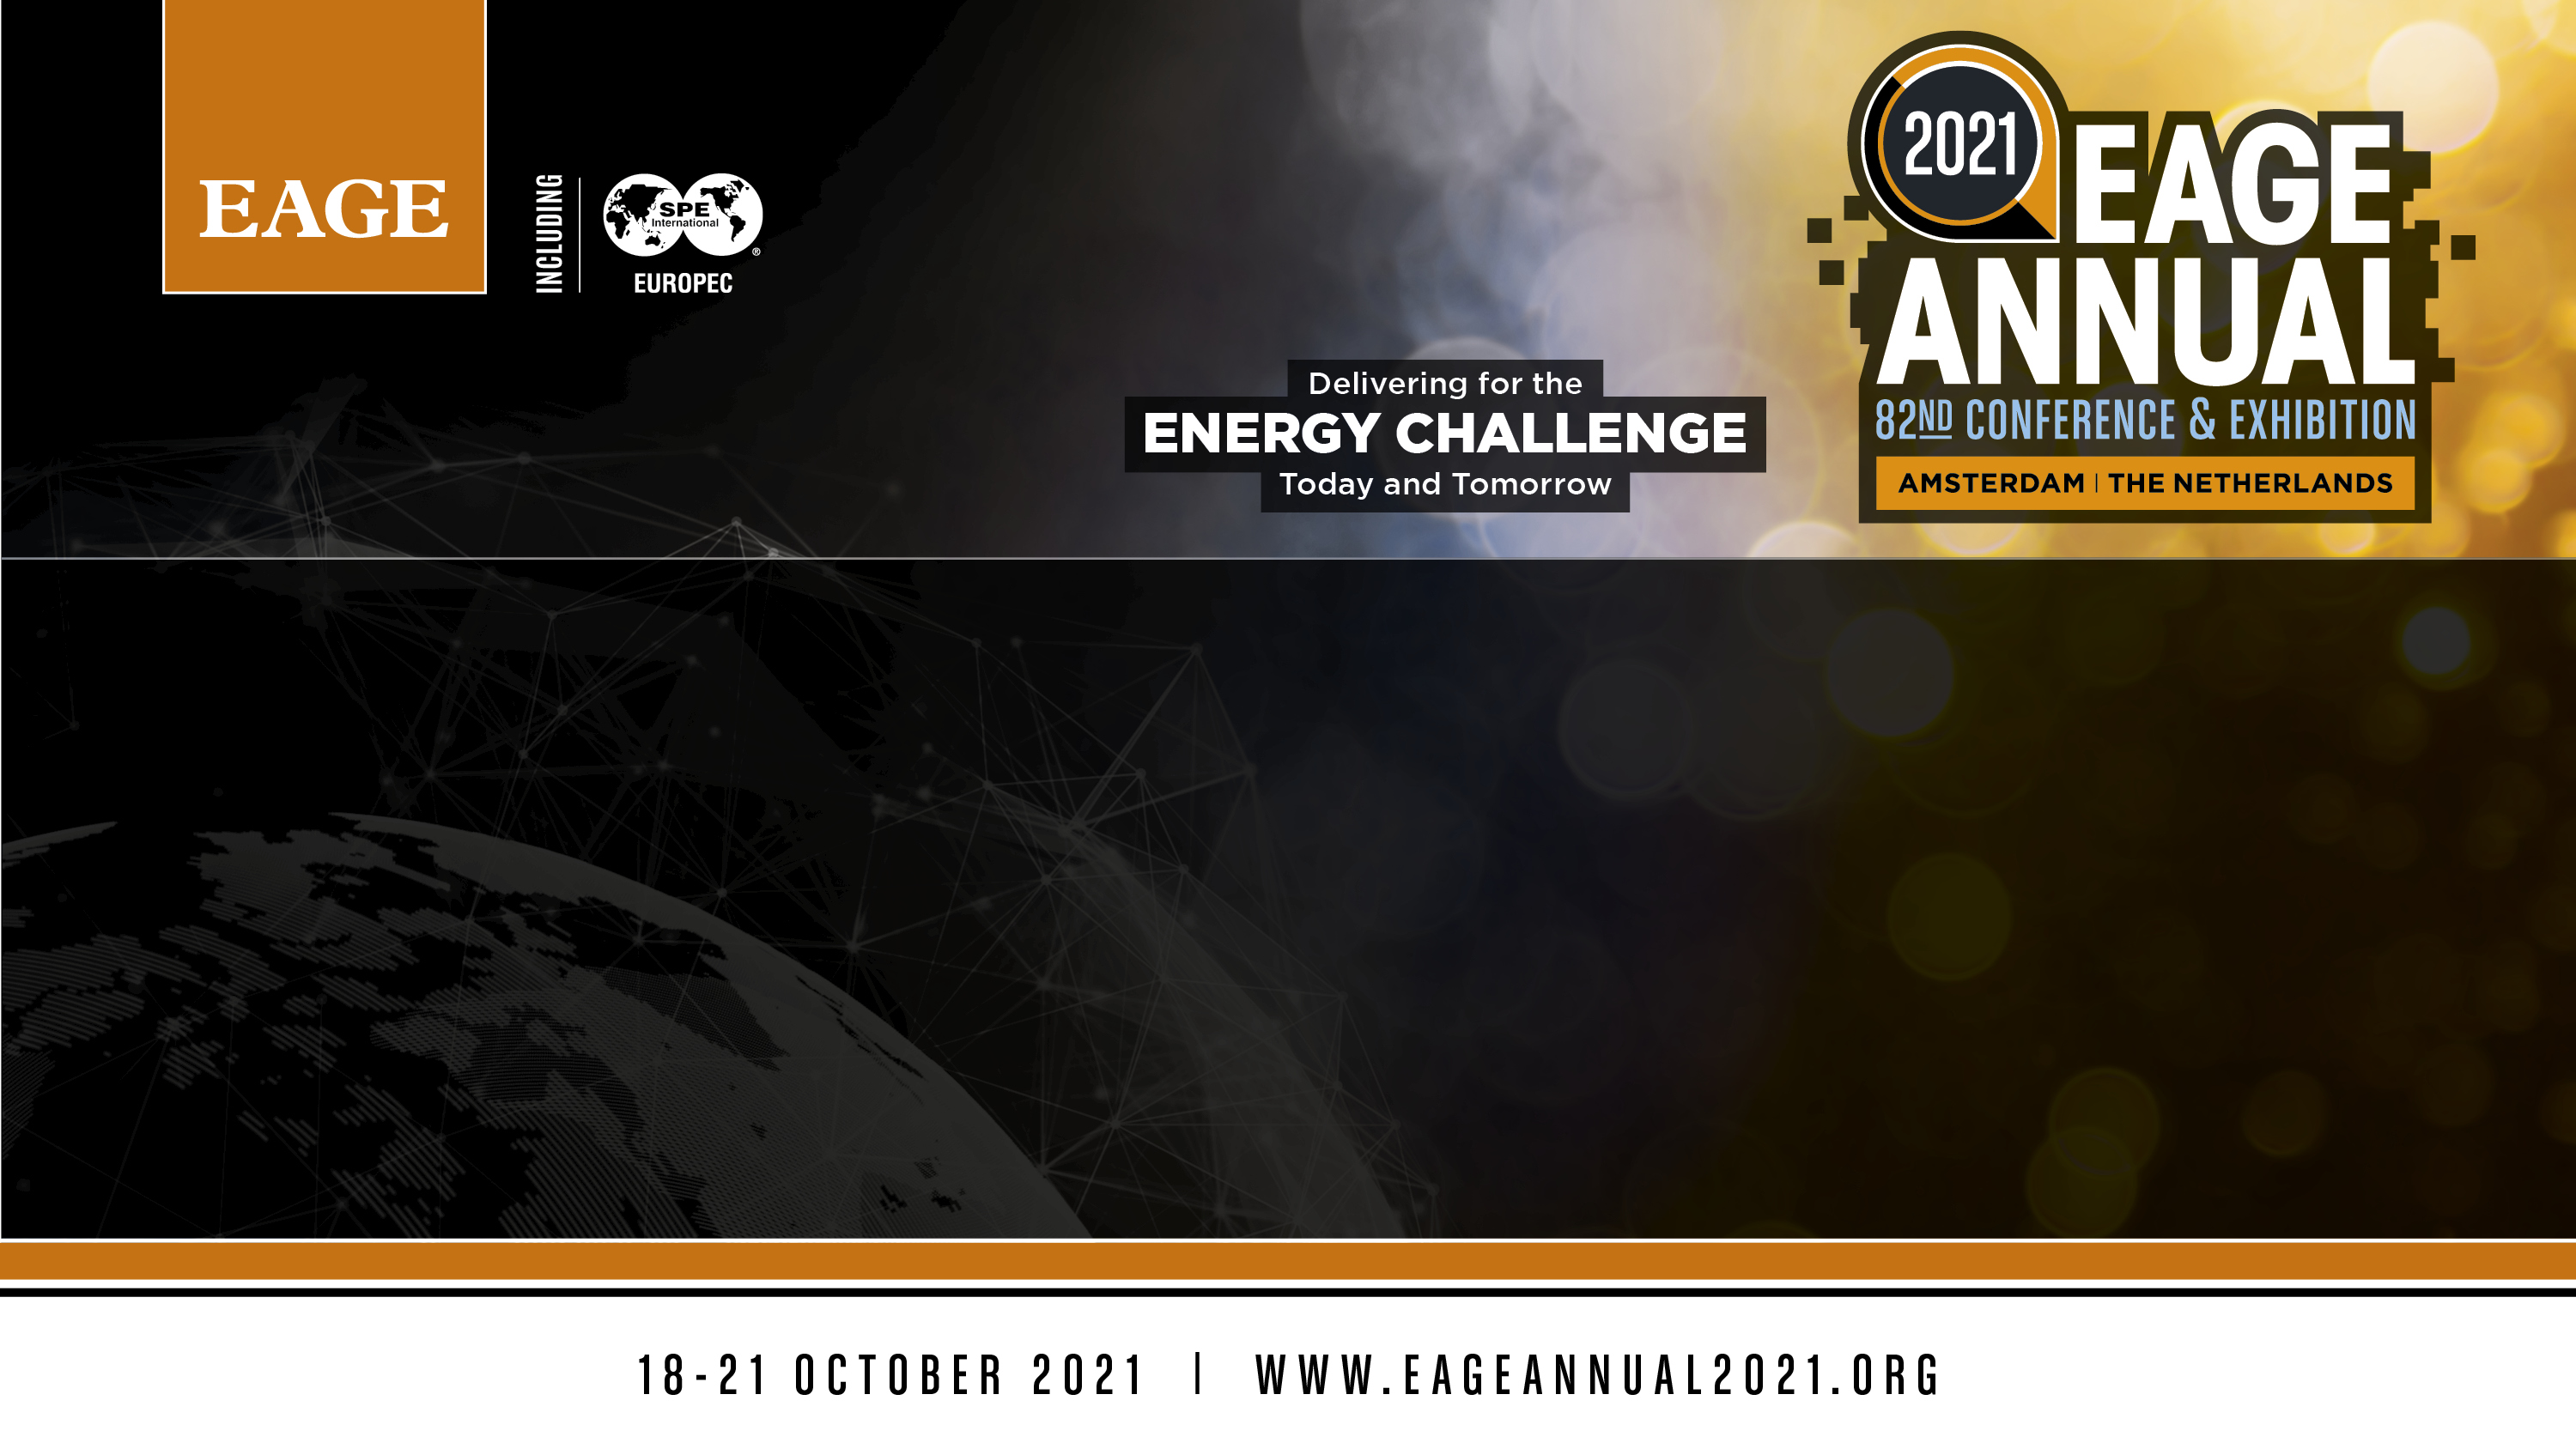
\includegraphics[width=\paperwidth]{SlideTitle}}

\maketitle % ---------------------------------------------------------------- %
\usebackgroundtemplate{
\includegraphics[width=\paperwidth]{SlideContent}}

\begin{frame}
  {Fast Fourier transform of EM data for computationally expensive kernels}

  \begin{itemize}
    \item Check and cite paper
    \item 15--25 frequencies
    \item Adaptive gridding; fct of skin depth
    \item Minimize frequencies; interpolation
    \item FFTLog or DLF
    \item Extrapolate, interpolate, set to zero
  \end{itemize}

  Either model in the domain of interest, or transform

  If transform, there are three key points:
  \begin{itemize}
    \item Solver
    \item Method and implementation of the transform
    \item Gridding
  \end{itemize}

  . The faster the solver, the faster modelling will be. It is important that
the solver is robust over a wide range of values (frequencies or times). The method should
require as few kernel evaluations as possible while remaining robust. As the frequency and
time ranges span many orders of magnitude, the required values are ideally equally spaced
on a logarithmic scale. The proposed fast method uses either the digital linear filter method
or the logarithmic fast Fourier transform together with a careful selection of evaluation points
and interpolation. In frequency-to-time domain tests this methodology requires typically 15–
20 frequencies to cover a wide range of offsets. The gridding should be frequency- or time-
dependent, which is accomplished by making it a function of skin depth. Optimizing for the
least number of required cells should be combined with optimizing for computational speed.
Looking carefully at these points resulted in much smaller computation times with speedup
factors of ten or more over previous methods. A computation in one domain followed by
transformation can therefore be an alternative to computation in the other domain domain if
the required evaluation points and the corresponding grids are carefully chosen.


This can significantly reduce the
computation time and makes time-domain CSEM modelling with
a frequency-domain code competitive given a robust frequency-
domain solver, a frequency-dependent gridding function that min-
imizes the required cells, and a Fourier transform that works on
a logarithmic scale.


\end{frame}

\begin{frame}
  {Example using FFTLog and Digital Linear Filters}
  \centering

  \bdra \quad (1) Frequency selection \quad (2) Gridding \quad \bdla\\[.5cm]

  First, show the important three points

  Show figure 1/2/3 of the paper. Forget the below ones.

  Then, show the actual timing results

  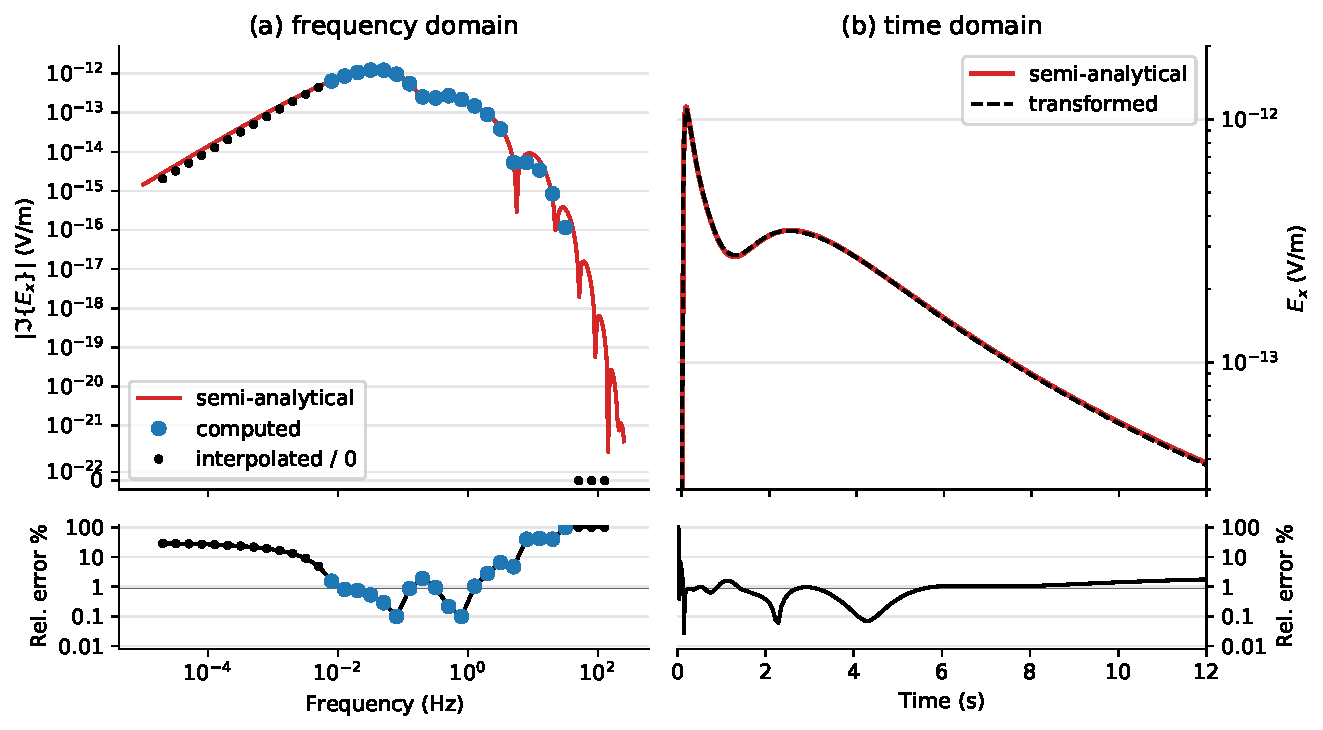
\includegraphics[width=.4\textwidth]{06-marine}
  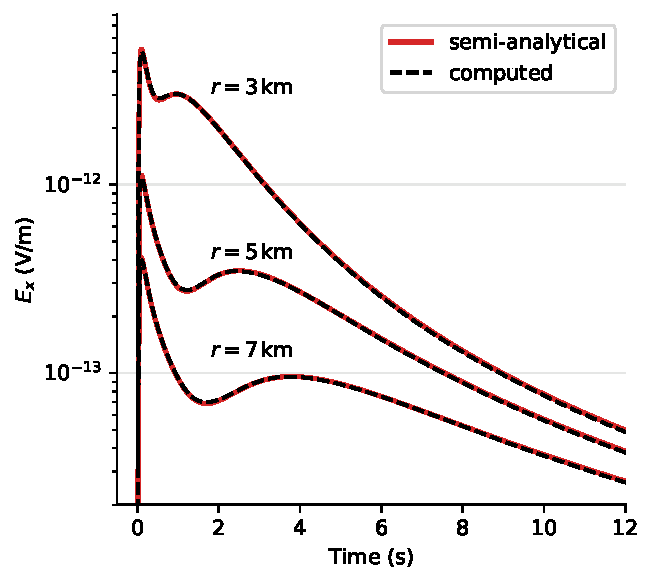
\includegraphics[width=.2\textwidth]{07-marine-multioffset}


  {\raggedright\small
  Werthmüller et al., 2021, \emph{Fast Fourier transform of electromagnetic
  data\\for computationally expensive kernels}, GJI; DOI:
  \href{https://doi.org/10.1093/gji/ggab171}{10.1093/gji/ggab171}.\\
  }


\end{frame}


\begin{frame}
  {Example: Induced Polarization}

  Also works for 3D or any model, as the transform is unaware of the
  complexity.

  27 frequencies instead of 747 frequencies (201\,pt filter)

  Tell what else they can find in the paper, and where they can find the paper
  (pure)

  \begin{columns}
    \column{.75\textwidth}
      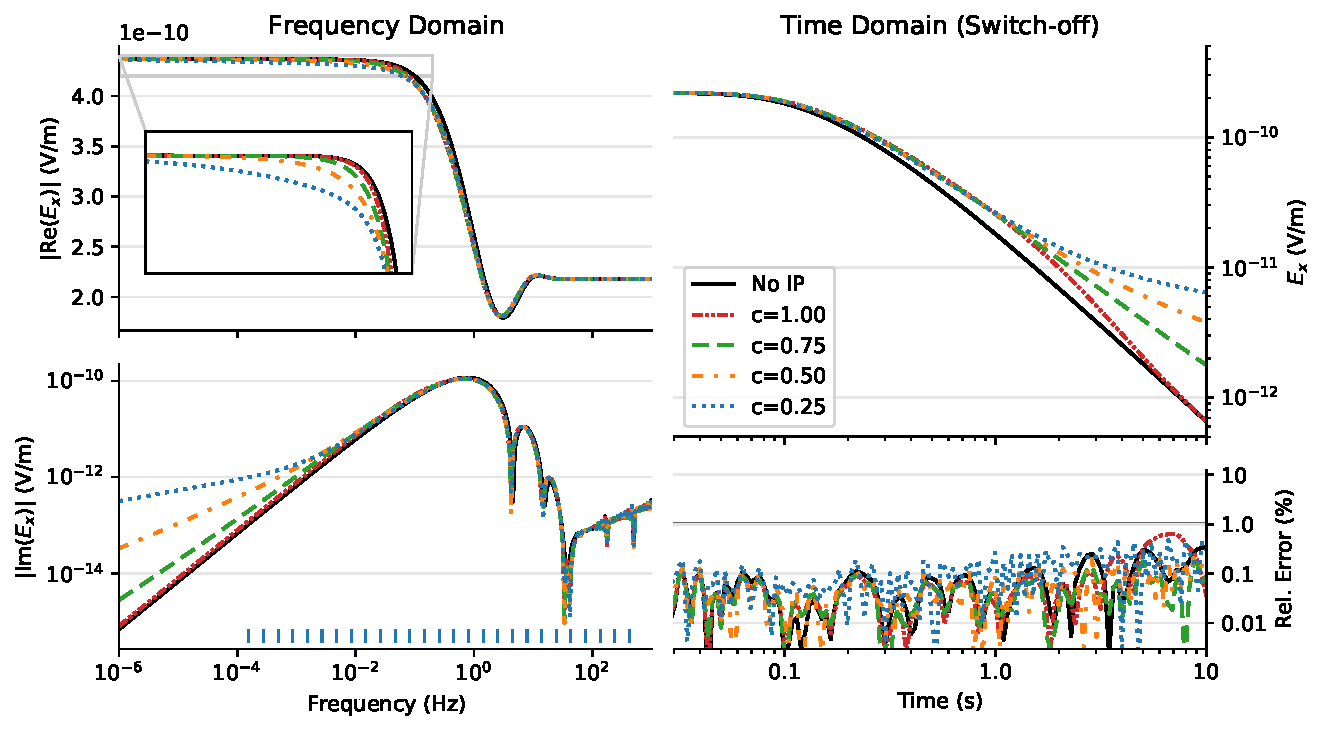
\includegraphics[width=\linewidth]{11-cole-cole-model}
    \column{.25\textwidth}
      %
      \begin{equation}
       ~\hspace{-.5cm} \sigma(\omega) = \sigma_\infty + \frac{\sigma_0 - \sigma_\infty}{1 +
          (\rm{i}\omega\tau)^c}
          \nonumber
      \end{equation}
      %
  \end{columns}

\end{frame}


\begin{frame}  % Motivation
  {Laplace-domain computation: Motivation}
  \centering
  \vspace{-.5cm}

  % Correct for: e^+iwt: + s σ E − ∇ × µ^-1 ∇ × E = − s J
  %              e^-iwt: + s σ E + ∇ × µ^-1 ∇ × E = − s J
  $$
    \mr{i}\omega \rightarrow s:
    \qquad
    \textcolor{red}{s} \sigma \mathbf{E} \ +\
    \nabla \times \mu^{-1} \nabla \times \mathbf{E}
    \ =\ -\textcolor{red}{s} \mathbf{J}_\mathrm{s}
  $$

  \bdra Faster\quad (1) Computation\quad (2) Convergence \quad \bdla\\
  \vspace{.5cm}

  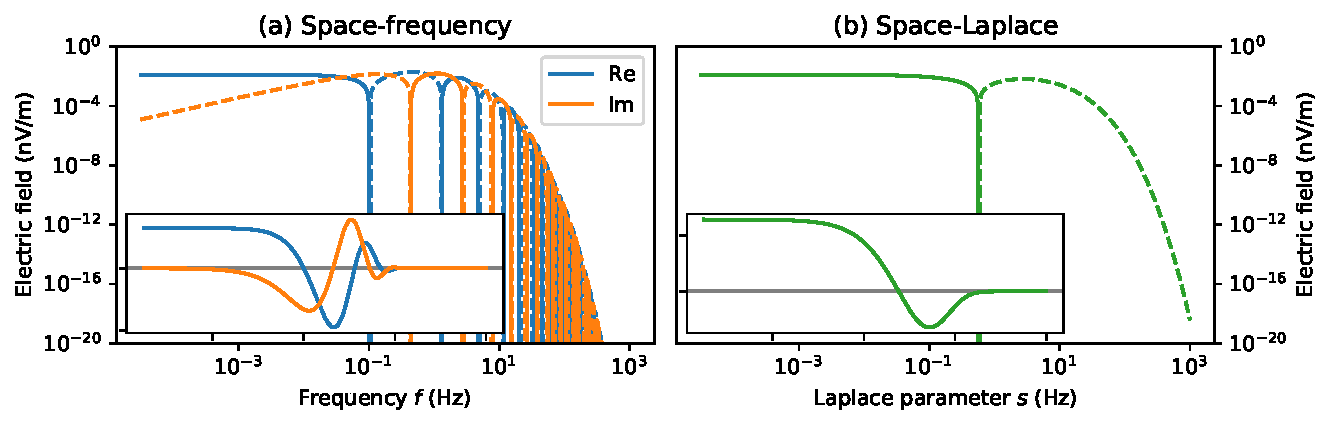
\includegraphics[width=\textwidth]{motivationcomparison}

\end{frame}

\begin{frame}  % Speed & Convergence
  {Computation in layered and 3D codes}

  \begin{itemize}
    \item 30\,\% speed up in computation \& convergence (?)
    \item Computation speed-up: 1D \& 3D; convergence speed-up only 3D
    \item Works for semi-analytical responses, but not otherwise
  \end{itemize}
\end{frame}

\begin{frame}  % Filter design
  {Digital linear filter for Laplace}
\end{frame}


\begin{frame}
  {1D example: works!}

  \begin{enumerate}
    \item Design digital linear filters for the transform
    \item Carry out transform for semi-analytical (layered) responses
    \item Test stability
  \end{enumerate}


  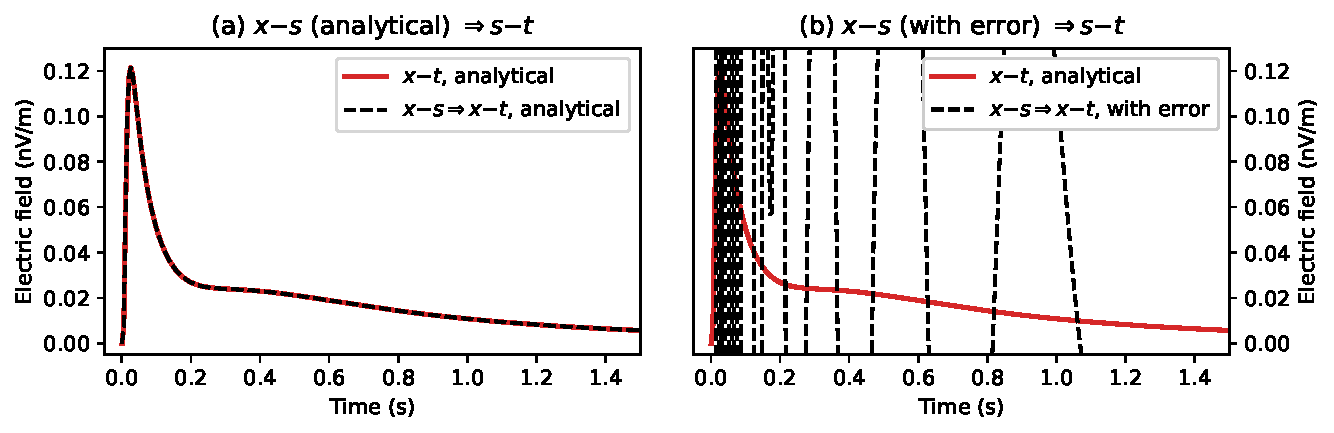
\includegraphics[width=\linewidth]{s-t_time}%

\end{frame}

\begin{frame}
  {1D example: it doesn't!}

  Only works for \emph{very} precise results.

\end{frame}


\begin{frame}
  {Laplace-to-frequency domain}

  Idea and filter

\end{frame}

\begin{frame}
  {s-f}

  Example
\end{frame}


\begin{frame}
  {Conclusions}:

  Note (\todo delete): 15 Minutes max \dra 15 slides max

  Conclusions
  \begin{itemize}
    \item f\dra t: 15-25 frequencies
    \item Laplace: xx speedup for computation and convergence
    \item s\dra t; s\dra f: Only works for very precise results.
  \end{itemize}
\end{frame}

\begin{frame}%
  {References}
  \begin{columns}
    \column{\textwidth}
  \setlength{\columnseprule}{0.4pt}
  % \setlength{\columnsep}{3em}
  \begin{multicols}{2}
  \tiny
  \begin{description}[2cm]
    %
    \item[Ghosh, D. P., 1971,] {\bfseries The application of linear filter
      theory to the direct interpretation of geoelectrical resistivity sounding
      measurements:} Geophysical Prospecting, 19, 192--217;
      \href{https://doi.org/10.1111/j.1365-2478.1971.tb00593.x}{doi:~10.1111/j.1365-2478.1971.tb00593.x}.
    %
    \item[Hamilton, A. J. S., 2000,] {\bfseries Uncorrelated modes of the
      non-linear power spectrum:} Monthly Notices of the Royal Astronomical
      Society, 312, pages 257--284;
      \href{https://doi.org/10.1046/j.1365-8711.2000.03071.x}%
      {doi:~10.1046/j.1365-8711.2000.03071.x}.
    %
    \item[Mulder, W. A., M. Wirianto, and E. Slob, 2008,] {\bfseries
      Time-domain modeling of electromagnetic diffusion with a
      frequency-domain code:} Geophysics, 73, F1--F8;
      \href{https://doi.org/10.1190/1.2799093}{doi:~10.1190/1.2799093}.
    %
    \item[Plessix, R.-E., M. Darnet, and W. A. Mulder, 2007,] {\bfseries An
      approach for 3D multisource, multifrequency CSEM modeling:} Geophysics,
      72, SM177--SM184;
      \href{https://doi.org/10.1190/1.2744234}{doi:~10.1190/1.2744234}.
    %
    \item[Werthmüller, D., 2017,] {\bfseries An open-source full 3D
        electromagnetic modeler for 1D VTI media in Python: empymod:}
        Geophysics, 82(6), WB9--WB19;
        \href{https://doi.org/10.1190/geo2016-0626.1}%
        {doi:~10.1190/geo2016-0626.1}.
    %
    \item[Werthmüller, D., K. Key, and E. C. Slob, 2019,] {\bfseries A tool
        for designing digital filters for the Hankel and Fourier transforms
        in potential, diffusive, and wavefield modeling:} Geophysics, 84(2),
        F47--F56; \href{https://doi.org/10.1190/geo2018-0069.1}%
        {doi:~10.1190/geo2018-0069.1}.
    %
    \item[Werthmüller, D., W. A. Mulder, and E. C. Slob, 2019,] {\bfseries
      emg3d: A multigrid solver for 3D electromagnetic diffusion:} Journal of
      Open Source Software, 4(39), 1463;
      \href{https://doi.org/10.21105/joss.01463}{doi:~10.21105/joss.01463}.
    %
    \item[Werthmüller, D., W. A. Mulder, and E. C. Slob, 2021,] {\bfseries Fast
      Fourier transform of electromagnetic data for computationally expensive
      kernels:} Geophysical Journal International, 226, No. 2, 1336--1347;
      \href{https://doi.org/10.1093/gji/ggab171}{doi:~10.1093/gji/ggab171}.
    %
  \end{description}
\end{multicols}
\end{columns}~\\[.1cm]


Used open-source codes: \empymod (layered models) \& \emg3d (3D models),
\href{https://emsig.xyz}{emsig.xyz}.

Acknowledgment:\\
\scriptsize
This research was conducted within the Gitaro.JIM project funded\\
through MarTERA as part of Horizon 2020 (ERA-NET Cofund).



\end{frame}

\end{document}
